\section{Introduction}

\subsection{History}

This package was born out of a $\approx$~10 line function I wrote to estimate 
the memory usage of (non-allocated) in-core, dense \proglang{R} objects of 
numeric (double precision) data.  I need this kind of thing for my 
work quite a bit, surprisingly, so it made sense to actually 
create this function instead of constantly doing ad hoc multiplications of 
$nrows\times ncols \times 8$ then dividing by powers of $1024$ (or 1000 --- 
more on this later).

But then I got the great idea to make this application \twiddle{enterprise 
ready} by adding a lot of unnecessary and convoluted OOP.  And so this 
stupid package was born.  From this perspective, this intentional 
(unnecessary) over-engineering is a sort of a love letter to other needlessly 
complex programs, like the 
\href{https://github.com/Mikkeren/FizzBuzzEnterpriseEdition}{Enterprise 
Fizzbuzz}\footnote{If you are unfamiliar with the 
\href{https://en.wikipedia.org/wiki/Bizz_buzz}{fizzbuzz}, see my posts ``\href{
http://librestats.com/2012/01/10/honing-your-r-skills-for-job-interviews/}{
Honing your R skills for Job Interviews}'' and 
``\href{http://librestats.com/2013/04/26/the-fizzbuzz-that-fortran-deserves/}{
The Fizzbuzz that Fortran Deserves}''.}.


\subsection{Purpose}

As hinted at in the above subsection, this package aids in the estimation of 
the memory usage of unallocated, dense, in-core, numeric objects; that's a 
very long-winded way of saying ``matrices'', but there you go.  So why should 
you care about this package?  Well, maybe you shouldn't; I'm not here to tell 
you what to do.  But this is an impressively useful little package for my own 
work, and possibly yours too. 
  
Aside from addressing uninteresting curiosities (e.g., \emph{How much ram do I 
need to store a $1,000,000\times 1,000$ matrix?} --- answer: about 7.5GiB), it 
is very handy when benchmarking, especially if you are doing any kind of 
scaling study. To be a bit loose, \emph{scalability} is the study of the 
performance of the implementation of a parallel algorithm.   Most people are 
fairly familiar with the concept of \emph{strong scalability}, even if they have 
never encountered the term before; this is where you try to capture how well 
your parallel algorithm is performing on a fixed total problem size, relative to 
the number of cores you throw at it.  Good scaling makes a kind of 
$y=\frac{1}{x}$ kind of plot, but is usually converted into a speedup plot, 
which frankly I don't really want to get into.  Look, I'm sorry I even brought 
it up, ok?

On the other hand, in a \emph{weak scaling} study, you 
keep the \emph{local} problem size (amount per processor) fixed and throw more 
cores at your method.  This is a much less known way of measuring performance 
for the \proglang{R} community, but it is a very useful one, especially when 
you break $\approx 10,000$ cores; at that scale, strong scalability generally 
isn't possible for any remotely interesting task.  The \pkg{memuse} package's 
methods \code{howbig()} and \code{howmany()} were designed with these two 
benchmarking tasks in mind.

In the remainder of the document, we will explore the \pkg{memuse} package, 
including how to install it, how to use it, and how it behaves with core 
\proglang{R} utilities.  Additionally, in the oh-so-cleverly titled
Section~\ref{howuse}, we will talk more about storage units for memory sizes 
than is reasonable.


\subsection{License}

\begin{figure}[th]
  \centering
  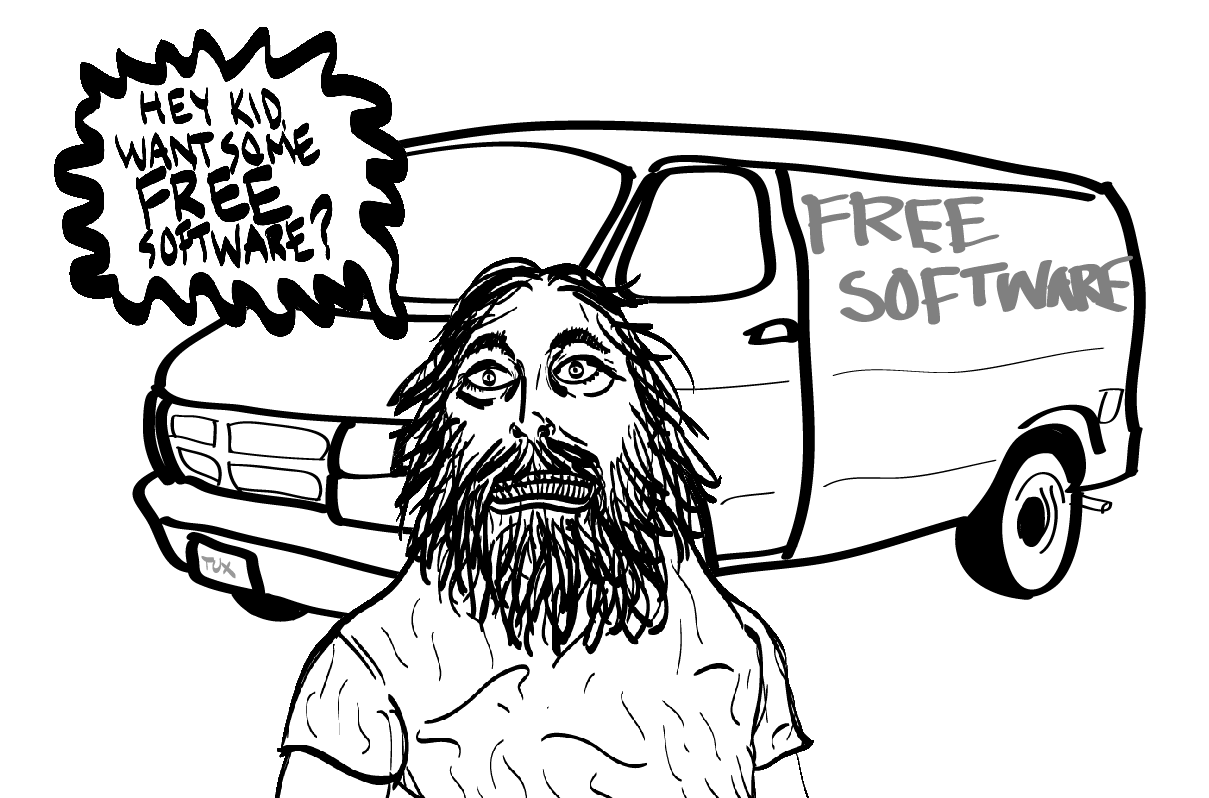
\includegraphics[scale=.35]{./include/gpl.png}
  \caption{The GNU GPL Explained}
  \label{fig:gnu}
\end{figure}

This package is libre software, or ``free and open source'', licensed under the 
GNU General Public License version $\geq$ 2 (see 
\hyperref[fig:gnu]{Figure~\ref{fig:gnu}} for full details).  If you 
violate the terms of the GPL, Richard Stallman's beard will sue you in 
internet court.